\documentclass[aspectratio=169,11pt]{beamer}

\usetheme{Madrid}
\usecolortheme{default}
\setbeamertemplate{navigation symbols}{}
\setbeamertemplate{footline}[frame number]

\definecolor{accent}{RGB}{30,80,150}
\setbeamercolor{structure}{fg=accent}
\setbeamercolor{frametitle}{bg=accent,fg=white}
\setbeamercolor{title}{fg=accent}
\setbeamertemplate{itemize items}[circle]

\usepackage{booktabs}
\usepackage{tikz}
\usetikzlibrary{arrows.meta,positioning}

\title{SkillOpt for AgentIA}
\subtitle{A bounded text-space optimization layer for procedural reliability}
\author{AgentIA Engineering}
\date{\today}

\begin{document}

\begin{frame}
  \titlepage
\end{frame}

\begin{frame}{The problem, in one sentence}
  AgentIA's failures are \textbf{procedural}, not capability gaps:
  the model \emph{knows} the rule (use \texttt{jakarta.*}; don't inject
  repositories into controllers) but forgets to apply it in a given
  session.

  \vspace{0.6em}
  \begin{block}{Two failure classes}
  \begin{itemize}
    \item \textbf{Capability gap} --- the model doesn't know the rule.
    No reminder helps.
    \item \textbf{Application gap} --- the model knows but doesn't apply.
    A persistent, triggered reminder helps.
  \end{itemize}
  \end{block}

  \vspace{0.4em}
  SkillOpt targets the second. It improves \emph{reliability within
  scope}, not coverage.
\end{frame}

\begin{frame}{What a skill actually is}
  Not a cheat sheet. A \textbf{procedural policy} with three parts:

  \begin{enumerate}
    \item \textbf{Trigger} --- \texttt{when\_to\_apply}
    \item \textbf{Procedure} --- ordered \texttt{rules}
    \item \textbf{Granularity} --- task-level or event-driven
  \end{enumerate}

  \vspace{0.6em}
  \begin{block}{Example (from CODESKILL's Java/Maven set)}
  \small
  \textbf{When.} A Maven build fails with a test-jar
  dependency-resolution error.\\
  \textbf{Rules.} Inspect the POM scope. Check the producing module for a
  plugin execution. Run tests or the test-jar goal explicitly. Do not
  retry with tests skipped. Run a full install. Verify presence before
  retrying.
  \end{block}

  \vspace{0.3em}
  At deployment: prepended to the generation prompt. Model stays frozen.
\end{frame}

\begin{frame}{What SkillOpt is}
  Treat the skill document as a \textbf{trainable parameter}. Build a
  training loop around it --- in text space, with the discipline of
  weight-space optimization.

  \vspace{0.8em}
  \begin{center}
  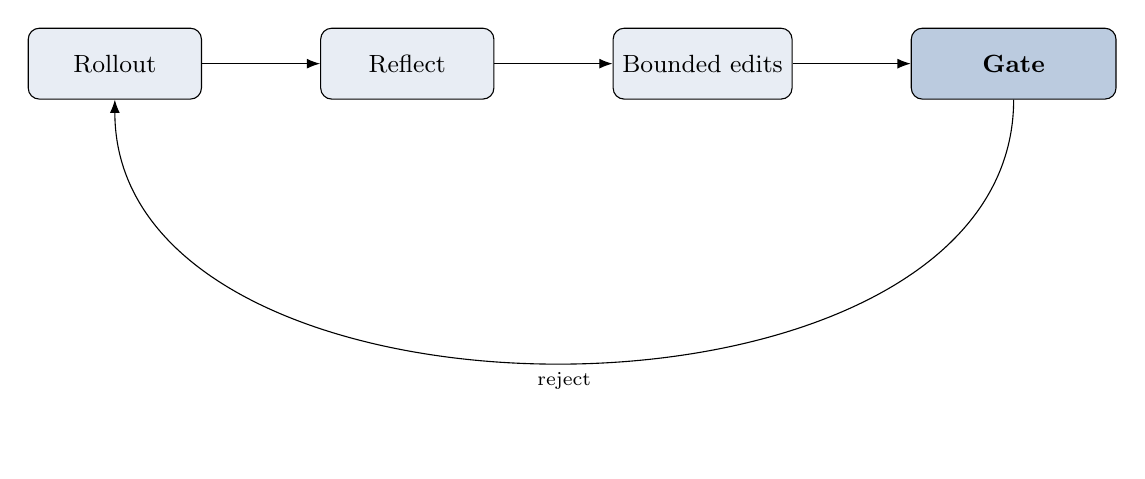
\begin{tikzpicture}[node distance=1.5cm, every node/.style={font=\small}]
    \node[draw, rounded corners, fill=accent!10, minimum width=2.2cm, minimum height=0.9cm] (roll) {Rollout};
    \node[draw, rounded corners, fill=accent!10, right=of roll, minimum width=2.2cm, minimum height=0.9cm] (refl) {Reflect};
    \node[draw, rounded corners, fill=accent!10, right=of refl, minimum width=2.2cm, minimum height=0.9cm] (edit) {Bounded edits};
    \node[draw, rounded corners, fill=accent!30, right=of edit, minimum width=2.6cm, minimum height=0.9cm] (gate) {\textbf{Gate}};
    \draw[-{Latex}] (roll) -- (refl);
    \draw[-{Latex}] (refl) -- (edit);
    \draw[-{Latex}] (edit) -- (gate);
    \draw[-{Latex}] (gate.south) to[out=-90,in=-90] node[below,font=\scriptsize]{reject} (roll.south);
  \end{tikzpicture}
  \end{center}

  \vspace{0.4em}
  Accepted only if the candidate \emph{strictly} improves a held-out
  score. Ties rejected.
\end{frame}

\begin{frame}{The four controls}
  \begin{description}
    \item[Bounded edit budget] $\le L_t$ edits per step
    (default $4$, cosine decay). Prevents unbounded rewriting.
    \item[Held-out validation gate] Accept iff selection score strictly
    improves. Makes the loop auditable and non-degrading.
    \item[Rejected-edit buffer] Failed edits fed back as negative
    evidence. Avoids repeated proposals.
    \item[Epoch-wise slow/meta update] Longitudinal guidance written to
    a protected section. Catches drift.
  \end{description}
\end{frame}

\begin{frame}{The loop}
  \begin{block}{Inner loop (per step)}
  \small
  rollout on training set $\to$ split success/failure $\to$ optimizer
  proposes edits $\to$ merge, dedupe, rank $\to$ clip to $L_t$ $\to$
  apply $\to$ \textbf{gate}.
  \end{block}

  \begin{block}{Outer loop (per epoch, 4 total)}
  \small
  sample 20 tasks $\to$ re-run under previous and current skill $\to$
  categorize $\to$ write longitudinal guidance to protected section
  $\to$ same gate.
  \end{block}

  \vspace{0.4em}
  \textbf{Output:} \texttt{best\_skill.md}, 300--2{,}000 tokens,
  inspectable, zero inference-time cost.
\end{frame}

\begin{frame}{The evidence}
  \begin{itemize}
    \item Best or tied-best on \textbf{52 of 52}
    (model, benchmark, harness) cells.
    \item GPT-5.5 direct chat: $+\,23.5$ pts over no-skill;
    Codex: $+\,24.8$; Claude Code: $+\,19.1$.
    \item Beats an \emph{oracle} per-cell baseline by $+\,5.4$ pts.
    \item \textbf{Edit economy:} 1--4 accepted edits produce $+\,29$ to
    $+\,39$ pts on procedural benchmarks.
    \item \textbf{Cross-harness transfer:} Codex-trained skill transfers
    to Claude Code at $+\,59.7$ over baseline.
  \end{itemize}
\end{frame}

\begin{frame}{The ablation that matters most}
  \begin{center}
  \begin{tabular}{@{}lcc@{}}
  \toprule
  Component & SpreadsheetBench & $\Delta$ \\
  \midrule
  Full SkillOpt & 77.5 & --- \\
  Without meta skill & 75.7 & $-1.8$ \\
  \textbf{Without meta + slow update} & \textbf{55.0} & $\mathbf{-22.5}$ \\
  \bottomrule
  \end{tabular}
  \end{center}

  \vspace{1em}
  The epoch-level longitudinal view is \textbf{load-bearing}, not
  decorative. Do not ship without it.
\end{frame}

\begin{frame}{Honest boundaries}
  \begin{itemize}
    \item \textbf{No code benchmark.} None of the six benchmarks is
    code. Mechanism is domain-agnostic; numbers do not transfer.
    \item \textbf{Requires an automated verifier.} The paper is
    explicit. \texttt{mvn test -o} satisfies this.
    \item \textbf{One document, not a bank.} Bank curation (SkillBrew,
    Ratchet) is deferred.
    \item \textbf{No weight changes.} No training infrastructure. That
    is a feature.
  \end{itemize}
\end{frame}

\begin{frame}{The staged plan}
  \begin{block}{Spec 1 --- inject and measure (1--2 weeks)}
  \small
  \begin{enumerate}
    \item \textbf{Task 0}: query \texttt{studio.db} for historical
    pass/fail and error classification. Triage domains.
    \item Hand-write seed skills for surviving domains.
    \item Add \texttt{skills} table, \texttt{skill\_injection\_node},
    injection logging, re-injection on repair.
    \item Four-condition A/B pilot ($\ge 15$ sessions per cell).
  \end{enumerate}
  \end{block}

  \begin{block}{Spec 2 --- optimize (4 weeks, conditional)}
  \small
  Full SkillOpt loop. Different-provider optimizer via
  \texttt{LLMFactory}. Only if Spec 1 shows signal.
  \end{block}
\end{frame}

\begin{frame}{The pilot design}
  \begin{table}
  \centering
  \small
  \begin{tabular}{@{}lll@{}}
  \toprule
  Condition & Prompt addition & Purpose \\
  \midrule
  \texttt{no\_skills} & none & Baseline \\
  \texttt{skills} & active skill docs & Treatment \\
  \texttt{sham} & $\sim$1.5K tokens of noise & Prompt-length control \\
  \texttt{skills\_plus\_fixer} & skills + fixer & Interaction \\
  \bottomrule
  \end{tabular}
  \end{table}

  \vspace{0.6em}
  \textbf{Primary metric:} \texttt{mvn test -o} pass rate.\\
  \textbf{Secondary:} reviewer tag (\texttt{as-is} / \texttt{minor} /
  \texttt{rewrite}).\\
  \textbf{Random assignment} within the same agent version and window.
\end{frame}

\begin{frame}{Decision points}
  \begin{enumerate}
    \item \textbf{After Task 0.} Which domains survive triage? Which
    go to deterministic fixers?
    \item \textbf{After Spec 1.} Does injection move the primary metric?
    If no, stop. If yes, build Spec 2.
    \item \textbf{Before Spec 2.} Spec 2 vs.\ coverage expansion
    (Spring Security). Equal footing. Not momentum.
  \end{enumerate}

  \vspace{0.8em}
  \begin{block}{The arithmetic worth stating}
  \small
  Reliability on 30--40\% of the requisition cannot reach a target
  defined against 100\% while 60--70\% is uncovered. Reliability is
  necessary infrastructure for coverage expansion --- not a substitute.
  \end{block}
\end{frame}

\begin{frame}{References}
  \small
  \begin{itemize}
    \item Li et al. \emph{SkillOpt: A controllable text-space optimizer
    for agent skills.} arXiv:2605.23904 (2026).
    \item Li et al. \emph{CODESKILL: Learning self-evolving skills for
    coding agents.} arXiv:2605.25430 (2026).
    \item Hu et al. \emph{SkillBrew: Multi-objective curation of skill
    banks for LLM agents.} arXiv:2605.29440 (2026).
    \item Eliseeva et al. \emph{EnvBench.} arXiv:2503.14443 (2025).
  \end{itemize}
\end{frame}

\end{document}